\documentclass[border=2pt]{standalone}
\usepackage{tikz}
\usetikzlibrary{shapes.symbols,positioning,arrows.meta}
\begin{document}
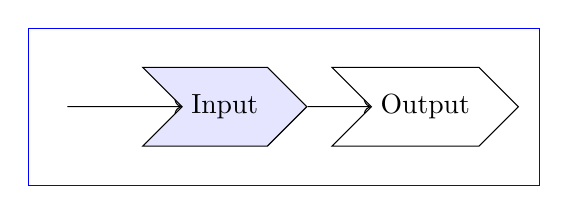
\begin{tikzpicture}[node distance=8mm]
  \draw[blue,line width=.2pt] (-2.5,-1) rectangle (4,1);
  \node[signal,signal from=west,signal to=east,signal pointer angle=90,
    minimum width=2cm,minimum height=1cm,draw,fill=blue!10] (input) {Input};
  \node[signal,signal from=west,signal to=east,minimum width=2cm,minimum height=1cm,
    draw,right=of input] (output) {Output};
  \draw[->] (-2,0) -- (input);
  \draw[->] (input) -- (output);
\end{tikzpicture}
\end{document}
